\documentclass{article}

\usepackage[margin=0.8in]{geometry}
\usepackage{polski}
\usepackage[utf8x]{inputenc}
\usepackage[hidelinks]{hyperref}
\usepackage{amsmath}
\usepackage{graphicx}
\usepackage[export]{adjustbox}
\usepackage{float}
\usepackage{subcaption}
\usepackage{color}
\usepackage{booktabs}

\hypersetup{
	colorlinks,
 	citecolor=black,
 	filecolor=black,
  	linkcolor=black,
  	urlcolor=black
}

\begin{document}

%	Main content
\section{Analiza metod modulacji PSK i APSK}
	\subsection{Próbka nr. 1, 64-PSK}
		Parametry testu:
		\begin{itemize}
			\item typ modulacji: 64-PSK,
			\item szum o rozkładzie normalnym,
			\item wariancja rozkładu: 0,05,
			\item liczebność próbki: 1000.
		\end{itemize}
		
		\subsubsection{Parametry dopasowanego do danych rozkładu normalnego}
			\begin{align*}
				&m = 	0,1072\\
				&\sigma = 0.0027
			\end{align*}
		
			\begin{figure}[H]
				\centering
				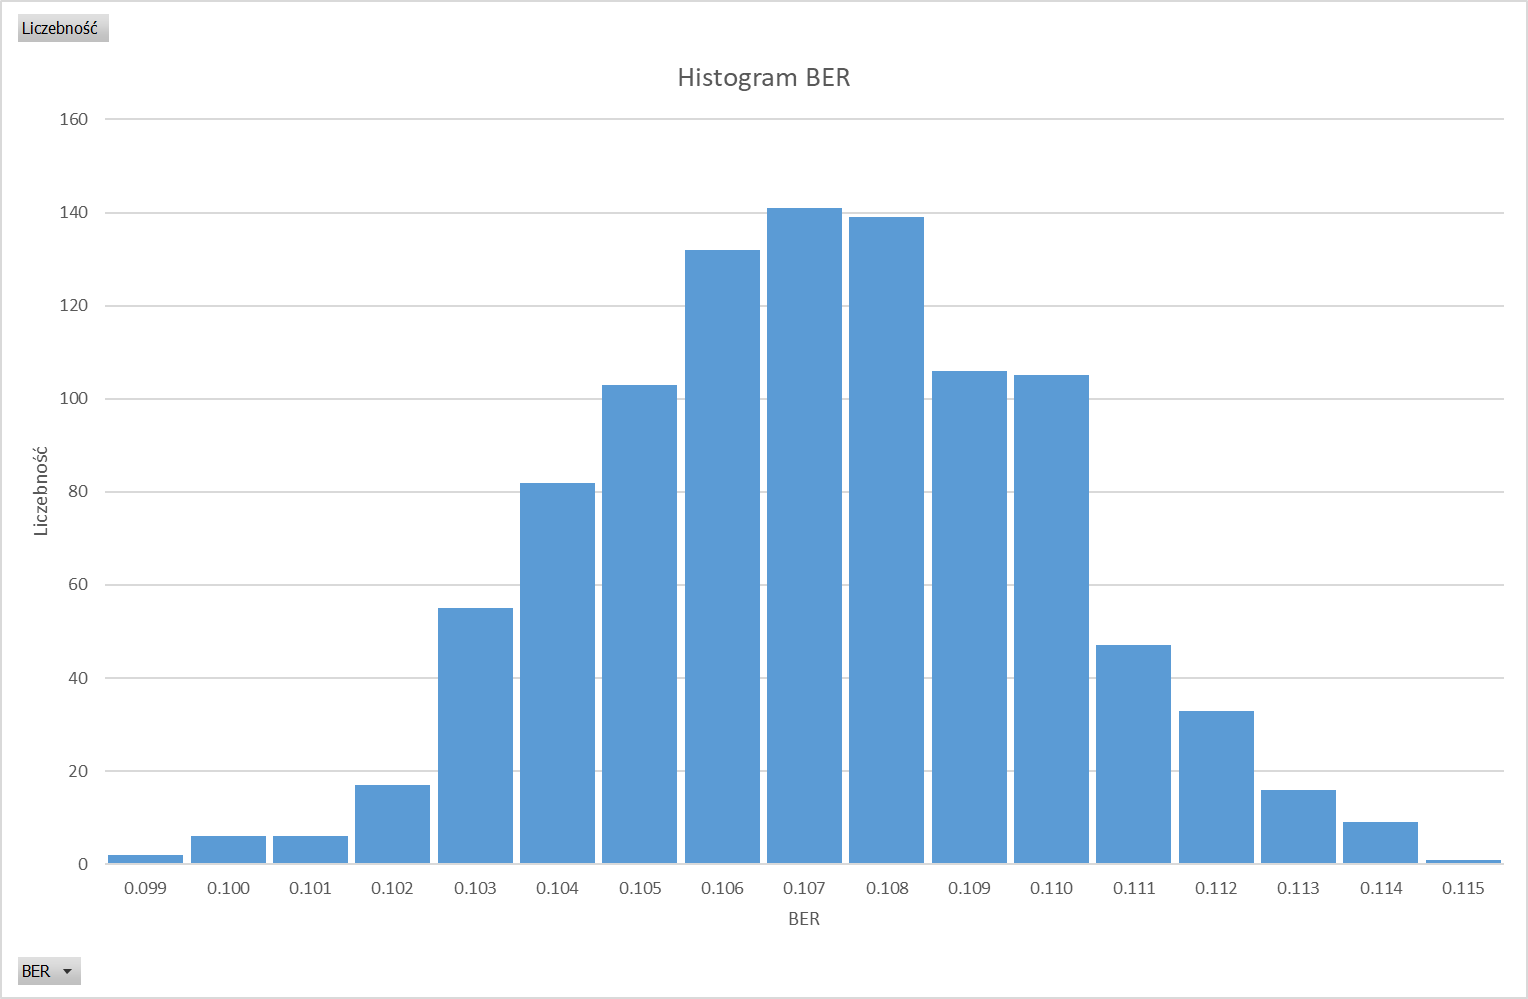
\includegraphics[width=0.8\linewidth]{img/hist_64psk005.png}
				\caption{Histogram}
			\end{figure}
			\begin{figure}[H]
				\centering
				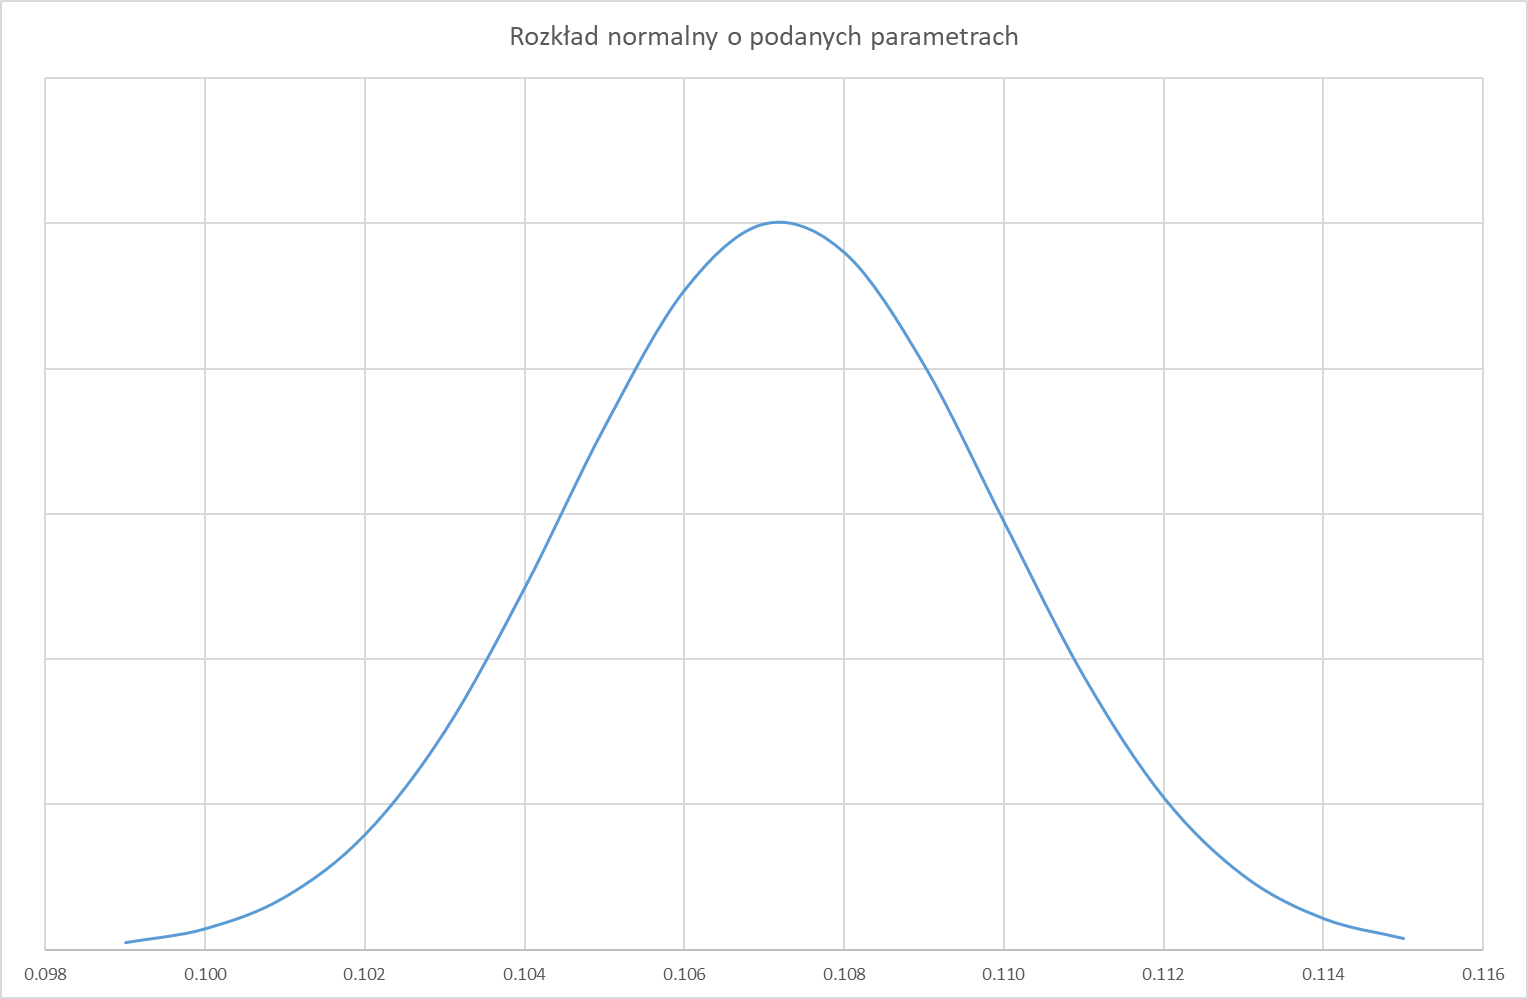
\includegraphics[width=0.8\linewidth]{img/rozk_64psk005.png}
				\caption{Rozkład normalny}
			\end{figure}
		
		\subsubsection{Analiza pięciopunktowa}
			\begin{table}[h]
				\begin{minipage}{0.5\linewidth}
					\caption{Tabela kwartyli}
					\label{table:student}
					\centering
					\begin{tabular}{lr}
						\toprule
						Kwartyl						& BER \\
						\midrule
						Q0 (minimum)		& 9,90\% \\
						Q1    							& 10,50\% \\
						Q2 (mediana)  		& 10,70\% \\
						Q3   							& 10,90\% \\
						Q4 (maksimum)	& 11,50\% \\
						\bottomrule
					\end{tabular}\\\vspace{5mm}
					$IQR = 0,40\%$
				\end{minipage}
				\begin{minipage}{0.45\linewidth}
					\centering
					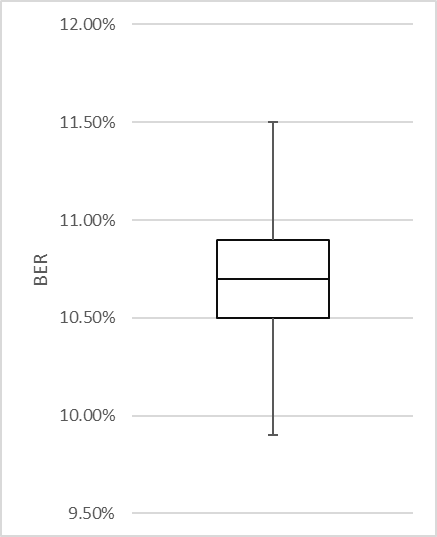
\includegraphics[width=0.8\linewidth]{img/five_64psk005.png}
					\captionof{figure}{Wykres wyników analizy pięciopunktowej}
					\label{ }
				\end{minipage}
			\end{table}

	\newpage
	\subsection{Próbka nr. 2, 64-PSK}
		Parametry testu:
		\begin{itemize}
			\item typ modulacji: 64-PSK,
			\item szum o rozkładzie normalnym,
			\item wariancja rozkładu: 0,1,
			\item liczebność próbki: 1000.
		\end{itemize}
		
		\subsubsection{Parametry dopasowanego do danych rozkładu normalnego}
			\begin{align*}
				&m = 	0,2061\\
				&\sigma = 0,00446
			\end{align*}
		
			\begin{figure}[H]
				\centering
				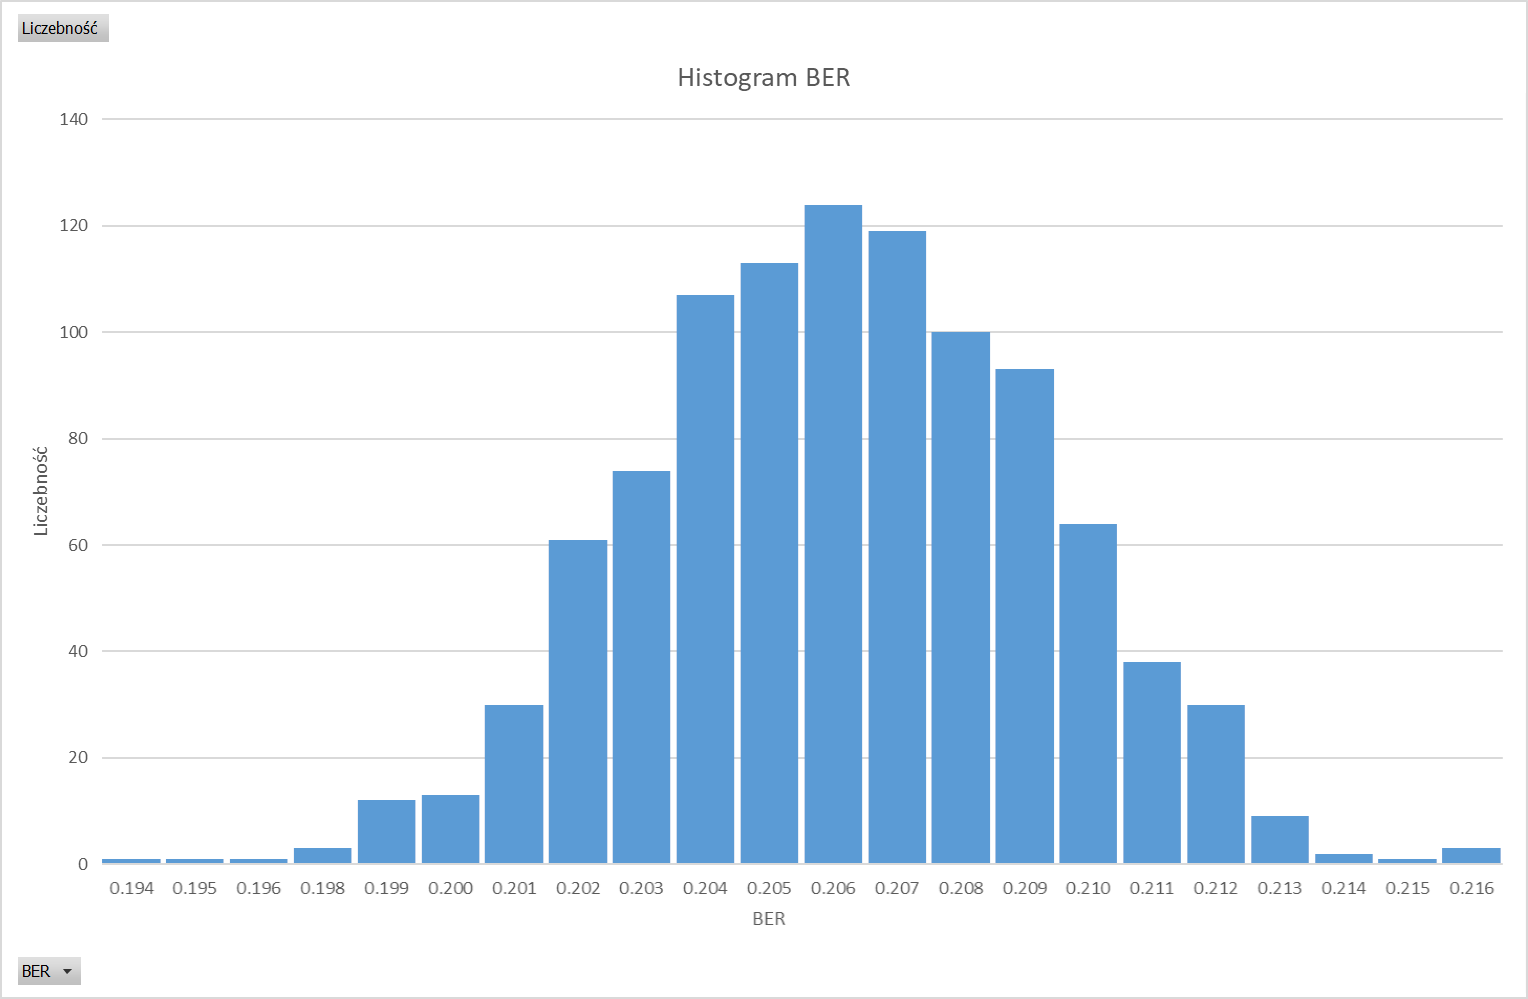
\includegraphics[width=0.8\linewidth]{img/hist_64psk01.png}
				\caption{Histogram}
			\end{figure}
			\begin{figure}[H]
				\centering
				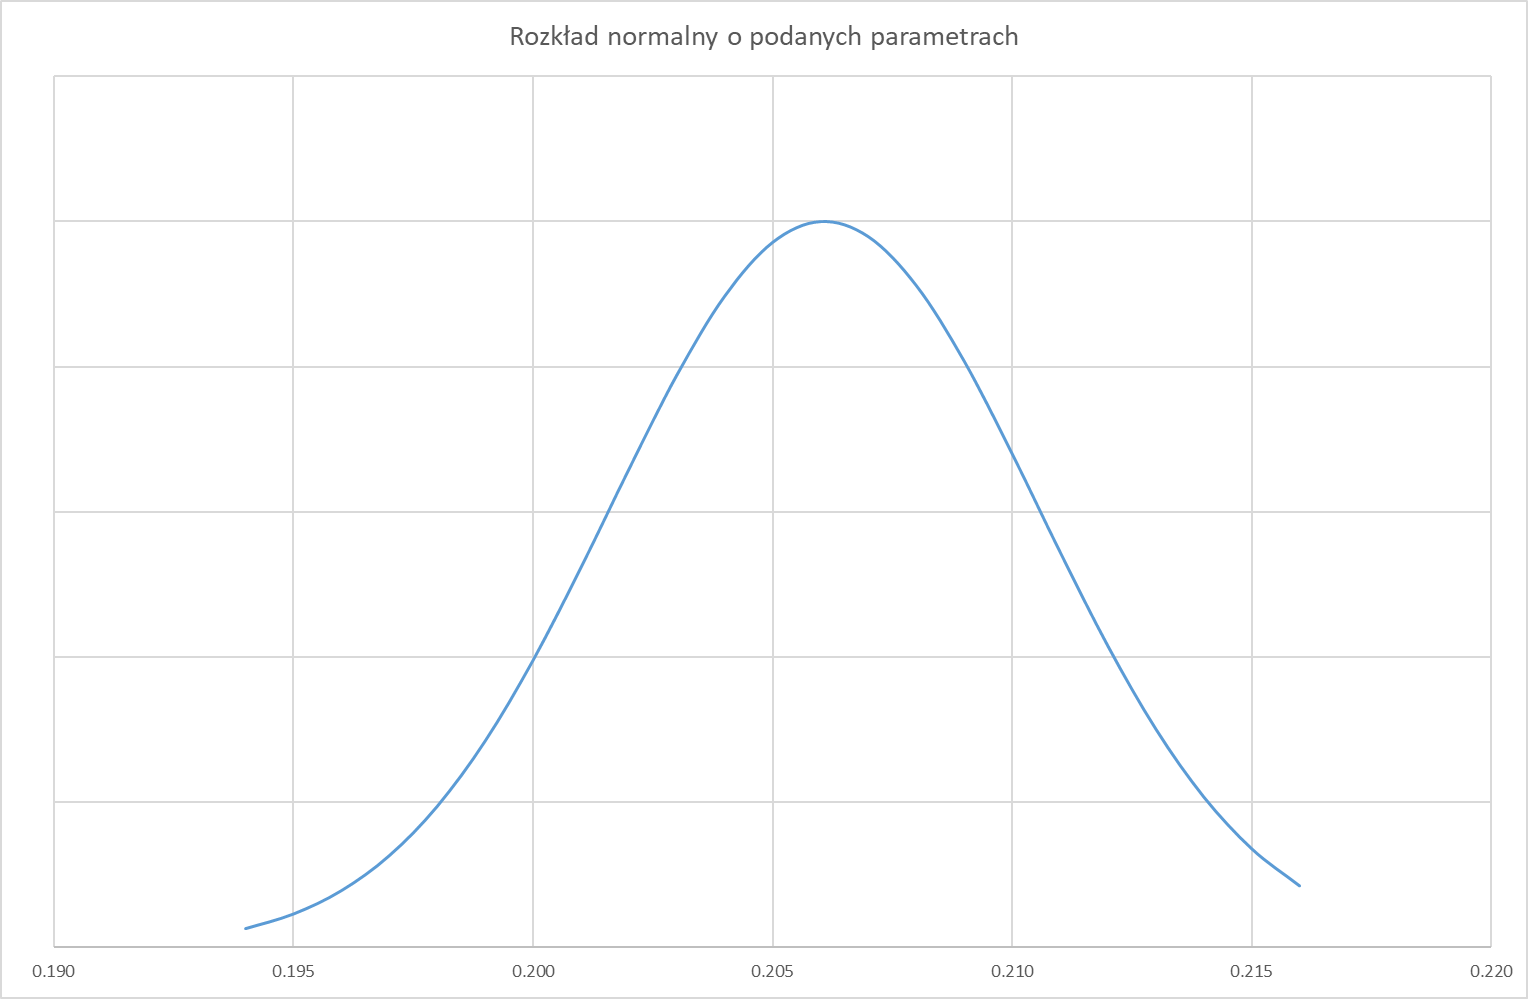
\includegraphics[width=0.8\linewidth]{img/rozk_64psk01.png}
				\caption{Rozkład normalny}
			\end{figure}
		
		\subsubsection{Analiza pięciopunktowa}
			\begin{table}[h]
				\begin{minipage}{0.5\linewidth}
					\caption{Tabela kwartyli}
					\label{table:student}
					\centering
					\begin{tabular}{lr}
						\toprule
						Kwartyl						& BER \\
						\midrule
						Q0 (minimum)		& 19,40\% \\
						Q1    							& 20,40\% \\
						Q2 (mediana)  		& 20,60\% \\
						Q3   							& 20,80\% \\
						Q4 (maksimum)	& 21,60\% \\
						\bottomrule
					\end{tabular}\\\vspace{5mm}
					$IQR = 0,40\%$
				\end{minipage}
				\begin{minipage}{0.45\linewidth}
					\centering
					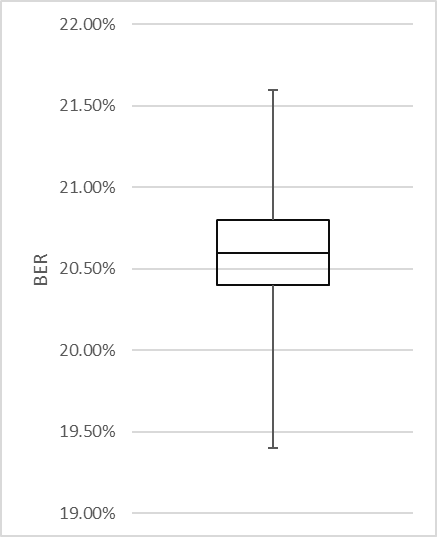
\includegraphics[width=0.8\linewidth]{img/five_64psk01.png}
					\captionof{figure}{Wykres wyników analizy pięciopunktowej}
					\label{ }
				\end{minipage}
			\end{table}
			
	\newpage
	\subsection{Próbka nr. 3, QPSK}
		Parametry testu:
		\begin{itemize}
			\item typ modulacji: QPSK,
			\item szum o rozkładzie normalnym,
			\item wariancja rozkładu: 0,7,
			\item liczebność próbki: 1000.
		\end{itemize}
		
		\subsubsection{Parametry dopasowanego do danych rozkładu normalnego}
			\begin{align*}
				&m = 0,2100\\
				&\sigma = 0,00285
			\end{align*}
		
			\begin{figure}[H]
				\centering
				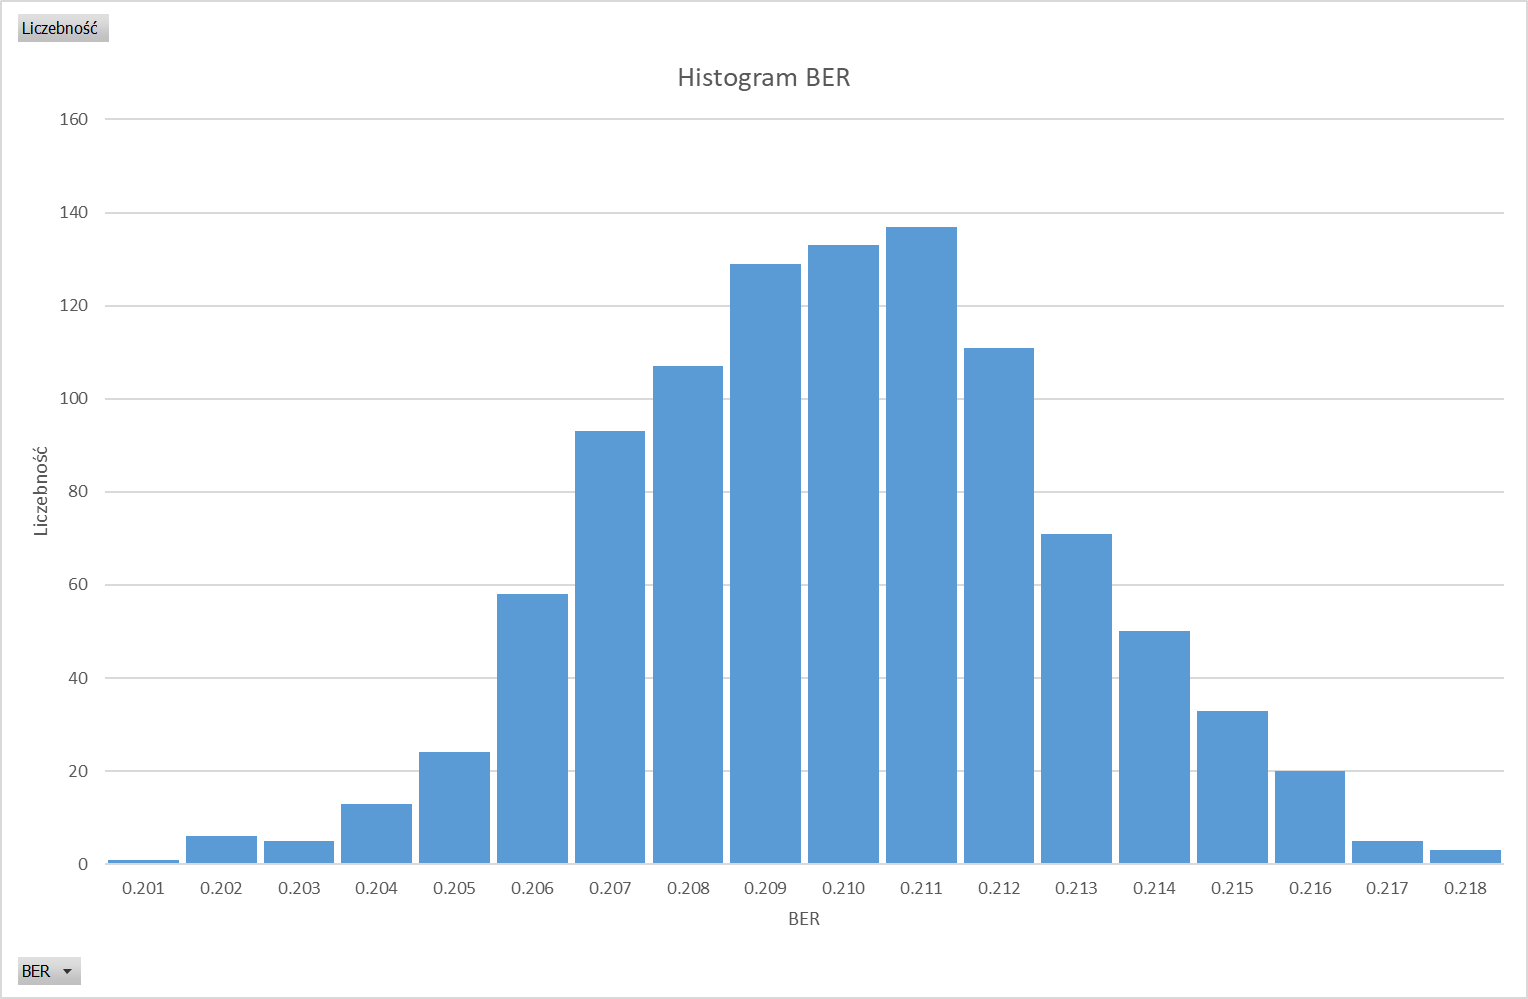
\includegraphics[width=0.8\linewidth]{img/hist_qpsk07.png}
				\caption{Histogram}
			\end{figure}
			\begin{figure}[H]
				\centering
				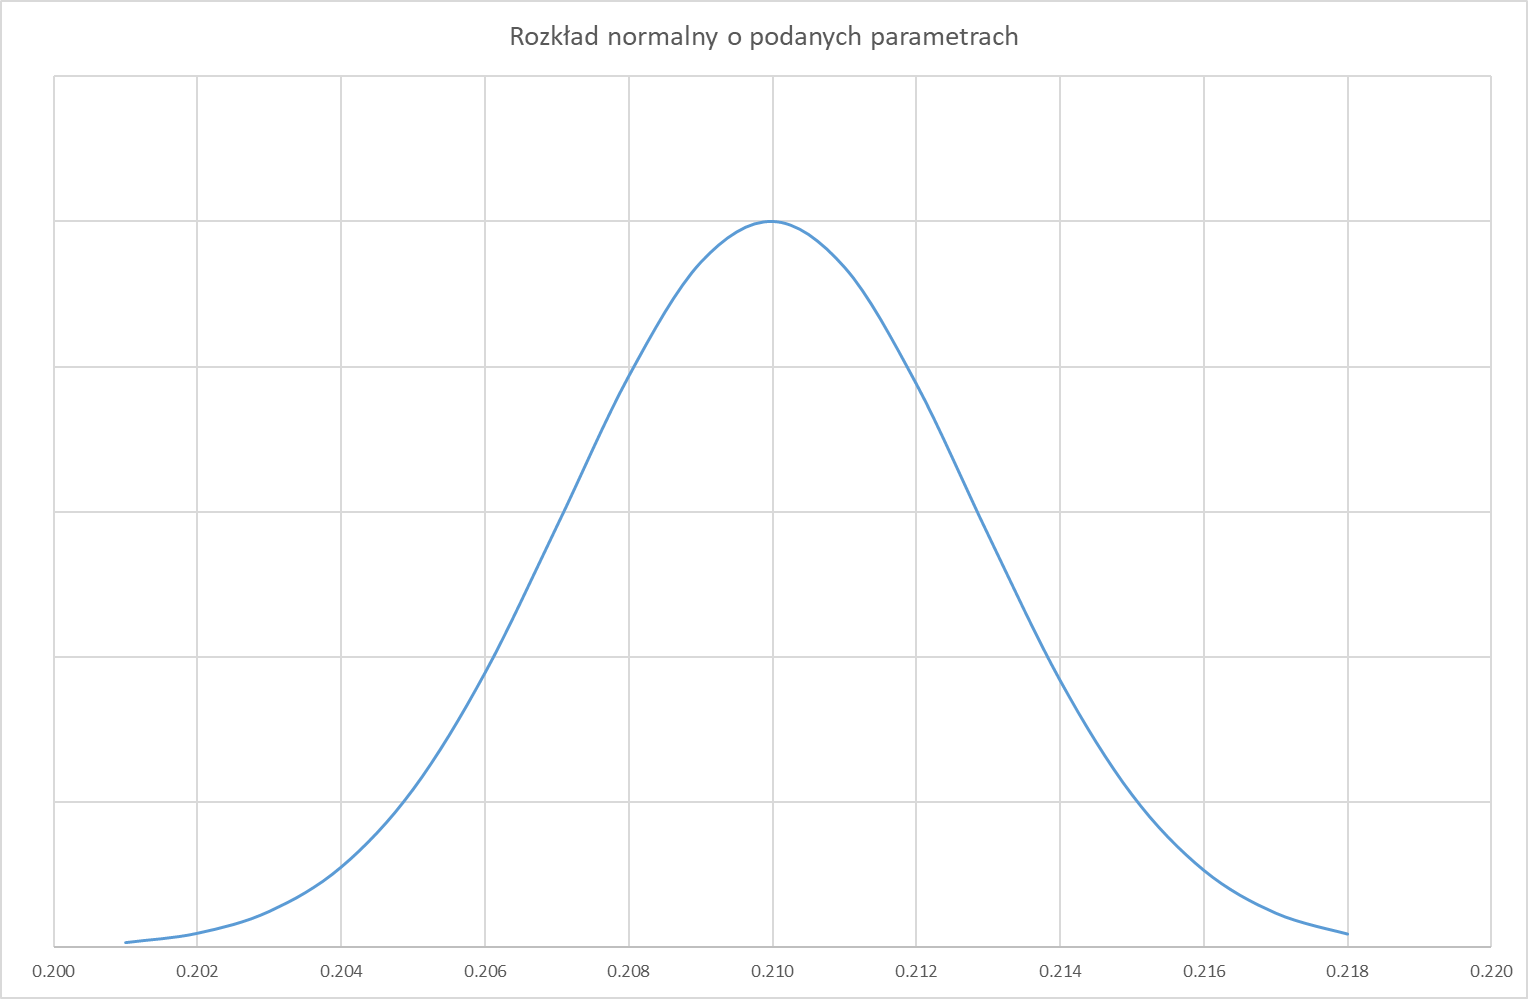
\includegraphics[width=0.8\linewidth]{img/rozk_qpsk07.png}
				\caption{Rozkład normalny}
			\end{figure}
		
		\subsubsection{Analiza pięciopunktowa}
			\begin{table}[h]
				\begin{minipage}{0.5\linewidth}
					\caption{Tabela kwartyli}
					\label{table:student}
					\centering
					\begin{tabular}{lr}
						\toprule
						Kwartyl						& BER \\
						\midrule
						Q0 (minimum)		& 20,10\% \\
						Q1    							& 20,80\% \\
						Q2 (mediana)  		& 21,00\% \\
						Q3   							& 21,20\% \\
						Q4 (maksimum)	& 21,80\% \\
						\bottomrule
					\end{tabular}\\\vspace{5mm}
					$IQR = 0,40\%$
				\end{minipage}
				\begin{minipage}{0.45\linewidth}
					\centering
					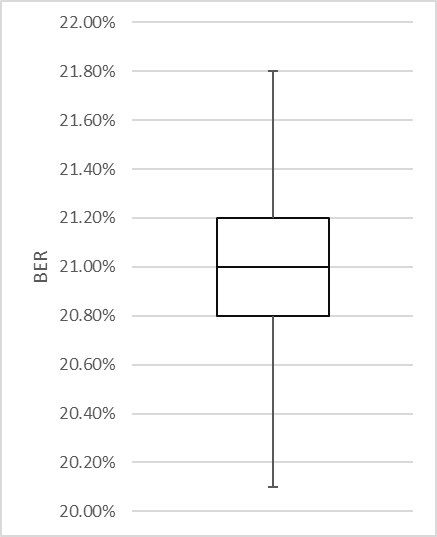
\includegraphics[width=0.8\linewidth]{img/five_qpsk07.png}
					\captionof{figure}{Wykres wyników analizy pięciopunktowej}
					\label{ }
				\end{minipage}
			\end{table}
			
	\newpage
	\subsection{Próbka nr. 4, QPSK}
		Parametry testu:
		\begin{itemize}
			\item typ modulacji: QPSK,
			\item szum o rozkładzie normalnym,
			\item wariancja rozkładu: 0,5,
			\item liczebność próbki: 1000.
		\end{itemize}
		
		\subsubsection{Parametry dopasowanego do danych rozkładu normalnego}
			\begin{align*}
				&m = 0,1118\\
				&\sigma = 0,00221
			\end{align*}
		
			\begin{figure}[H]
				\centering
				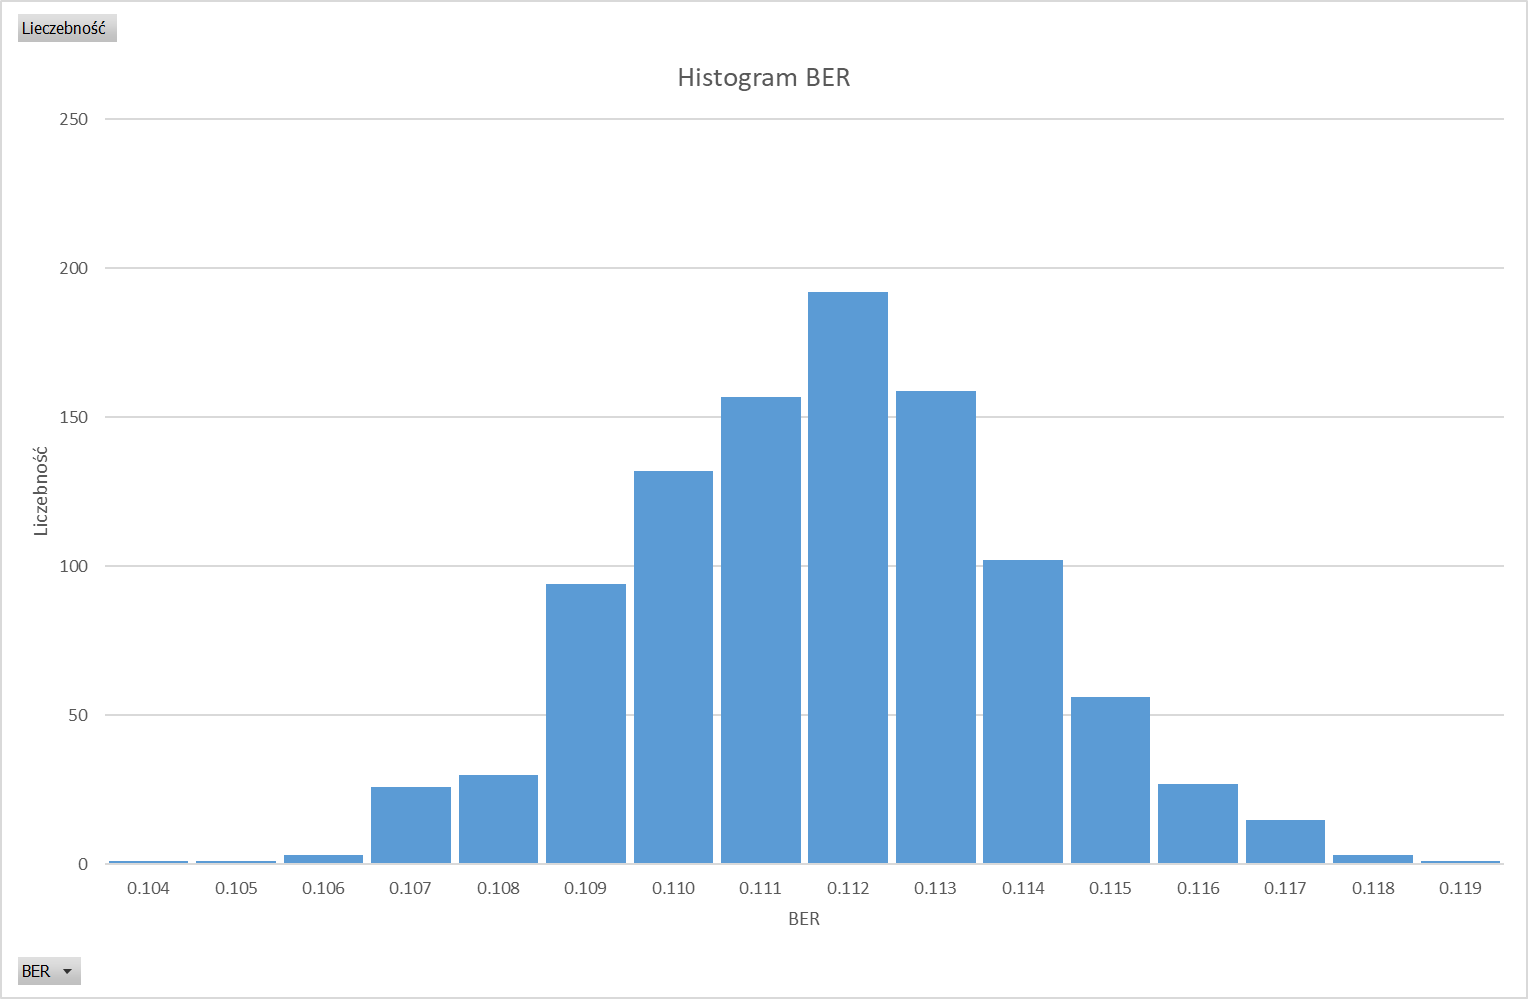
\includegraphics[width=0.8\linewidth]{img/hist_qpsk05.png}
				\caption{Histogram}
			\end{figure}
			\begin{figure}[H]
				\centering
				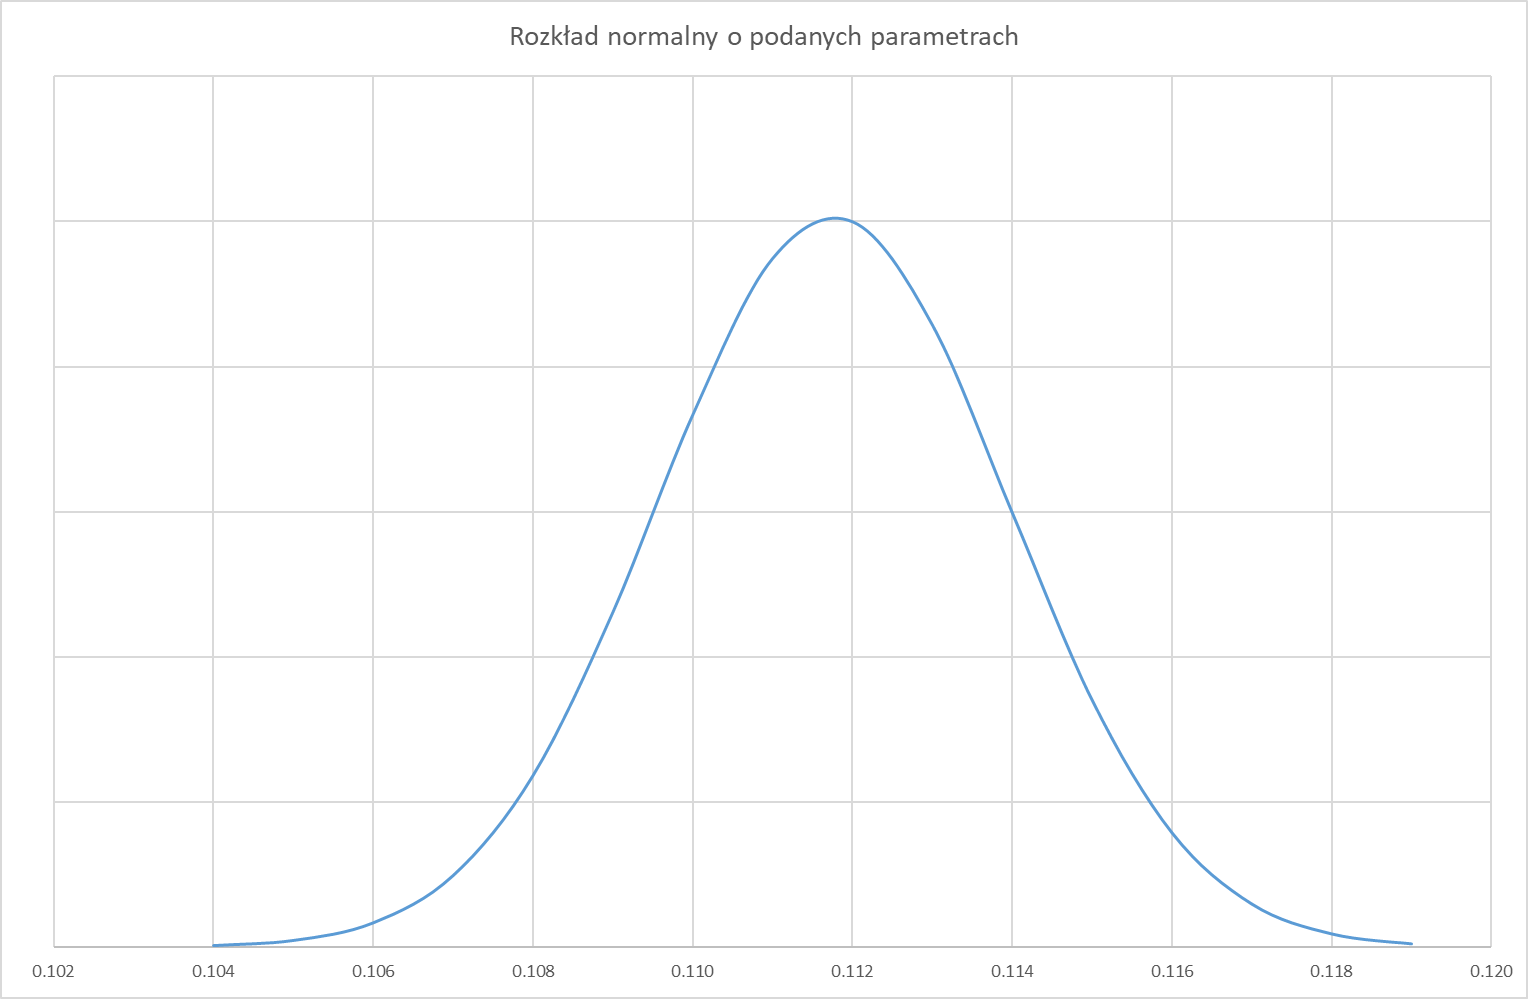
\includegraphics[width=0.8\linewidth]{img/rozk_qpsk05.png}
				\caption{Rozkład normalny}
			\end{figure}
		
		\subsubsection{Analiza pięciopunktowa}
			\begin{table}[h]
				\begin{minipage}{0.5\linewidth}
					\caption{Tabela kwartyli}
					\label{table:student}
					\centering
					\begin{tabular}{lr}
						\toprule
						Kwartyl						& BER \\
						\midrule
						Q0 (minimum)		& 10,10\% \\
						Q1    							& 11,00\% \\
						Q2 (mediana)  		& 11,20\% \\
						Q3   							& 11,30\% \\
						Q4 (maksimum)	& 11,90\% \\
						\bottomrule
					\end{tabular}\\\vspace{5mm}
					$IQR = 0,30\%$
				\end{minipage}
				\begin{minipage}{0.45\linewidth}
					\centering
					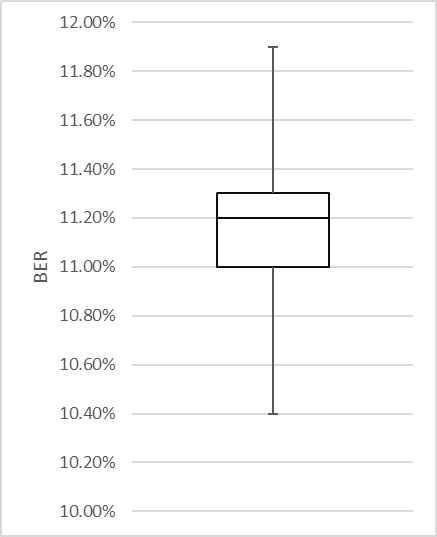
\includegraphics[width=0.8\linewidth]{img/five_qpsk05.png}
					\captionof{figure}{Wykres wyników analizy pięciopunktowej}
					\label{ }
				\end{minipage}
			\end{table}

\end{document}